\documentclass[a4paper,11pt]{article}
\usepackage{amsmath,amsthm,amsfonts,amssymb,amscd,amstext,vmargin,graphics,graphicx,tabularx,multicol} 
\usepackage[francais]{babel}
\usepackage[utf8]{inputenc}  
\usepackage[T1]{fontenc} 
\usepackage{pstricks-add,tikz,tkz-tab,variations}
\usepackage[autolanguage,np]{numprint} 

\setmarginsrb{1.5cm}{0.5cm}{1cm}{0.5cm}{0cm}{0cm}{0cm}{0cm} %Gauche, haut, droite, haut
\newcounter{numexo}
\newcommand{\exo}[1]{\stepcounter{numexo}\noindent{\bf \underline{Exercice~\thenumexo}}}
\reversemarginpar


\newcounter{enumtabi}
\newcounter{enumtaba}
\newcommand{\q}{\stepcounter{enumtabi} \theenumtabi.  }
\newcommand{\qa}{\stepcounter{enumtaba} (\alph{enumtaba}) }
\newcommand{\initq}{\setcounter{enumtabi}{0}}
\newcommand{\initqa}{\setcounter{enumtaba}{0}}

\newcommand{\be}{\begin{enumerate}}
\newcommand{\ee}{\end{enumerate}}
\newcommand{\bi}{\begin{itemize}}
\newcommand{\ei}{\end{itemize}}
\newcommand{\bp}{\begin{pspicture*}}
\newcommand{\ep}{\end{pspicture*}}
\newcommand{\bt}{\begin{tabular}}
\newcommand{\et}{\end{tabular}}
\renewcommand{\tabularxcolumn}[1]{>{\centering}m{#1}} %(colonne m{} centrée, au lieu de p par défault) 
\newcommand{\tnl}{\tabularnewline}

\newcommand{\bmul}[1]{\begin{multicols}{#1}}
\newcommand{\emul}{\end{multicols}}

\newcommand{\trait}{\noindent \rule{\linewidth}{0.2mm}}
\newcommand{\hs}[1]{\hspace{#1}}
\newcommand{\vs}[1]{\vspace{#1}}

\newcommand{\N}{\mathbb{N}}
\newcommand{\Z}{\mathbb{Z}}
\newcommand{\R}{\mathbb{R}}
\newcommand{\C}{\mathbb{C}}
\newcommand{\Dcal}{\mathcal{D}}
\newcommand{\Ccal}{\mathcal{C}}
\newcommand{\mc}{\mathcal}

\newcommand{\vect}[1]{\overrightarrow{#1}}
\newcommand{\ds}{\displaystyle}
\newcommand{\eq}{\quad \Leftrightarrow \quad}
\newcommand{\vecti}{\vec{\imath}}
\newcommand{\vectj}{\vec{\jmath}}
\newcommand{\Oij}{(O;\vec{\imath}, \vec{\jmath})}
\newcommand{\OIJ}{(O;I,J)}




\newcommand{\reponse}[1][1]{%
\multido{}{#1}{\makebox[\linewidth]{\rule[0pt]{0pt}{20pt}\dotfill}
}}

\newcommand{\titre}[5] 
% #1: titre #2: haut gauche #3: bas gauche #4: haut droite #5: bas droite
{
\noindent #2 \hfill #4 \\
#3 \hfill #5

\vspace{-1.6cm}

\begin{center}\rule{6cm}{0.5mm}\end{center}
\vspace{0.2cm}
\begin{center}{\large{\textbf{#1}}}\end{center}
\begin{center}\rule{6cm}{0.5mm}\end{center}
}



\begin{document}
\pagestyle{empty}
\titre{Chapitre 7 : Règle, équerre et compas}{}{}{}{}

\vspace*{1cm}

\begin{center}
{\Large \textbf{Niveau 1 :}}
\end{center}

\vspace*{1cm}

$\rightarrow$ \textbf{Notations et vocabulaire}\\

\vspace*{0.5cm}


\exo \\ Compléter la définition d'un point. \\

Un point du plan est un lieu, un endroit qui n'a ni longueur ni épaisseur. \\
On note un point avec . . . . . . . . . . . . . . . . . . . . . . . . . . .\\ Sur une feuille, on note l'endroit où il se trouve par une . . . . . . . . . . .\\


\exo \\ Compléter la définition d'un segment. \\

Un segment est une ligne droite . . . . . . . . . . . des deux côtés par ses . . . . . . . . . . . . . . . . . .\\


\exo \\ Indiquer le nom du segment en gras sur chaque figure.\\

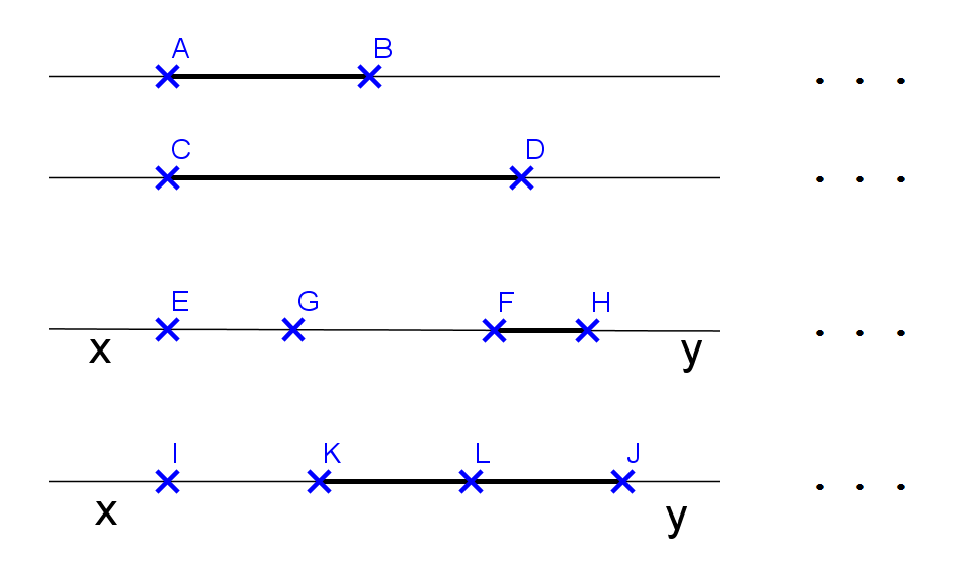
\includegraphics[scale=0.95]{notation2.eps} \\

\exo \\ Quel(s) est/sont le(s) point(s) correctement représenté(s) parmi ceux dessinés ci-dessous.\\

\begin{center}
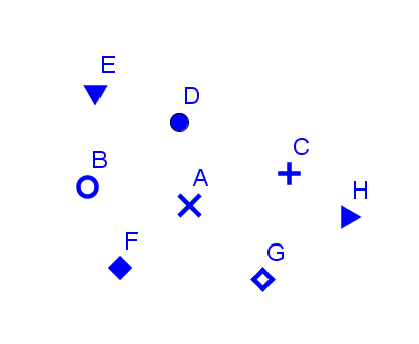
\includegraphics[scale=0.95]{notation3.eps} 
\end{center}

Réponse : . . . . . . . . . . . . . .\\

\vspace*{1cm}

$\rightarrow$ \textbf{DROITES PARALLÈLES ET PERPENDICULAIRES : Savoir reconnaître des droites parallèles et perpendiculaires}\\

\vspace*{0.5cm}


\exo \\ Compléter la définition de deux droites sécantes. \\

On dit que deux droites (d) et (d') sont sécantes lorsqu'elles ont . . . . . . . . . . . . . . . . . . . .  . . . . . . . . . . . . .\\
On appelle alors ce point leur . . . . . . . . . . . . . . . . . . . . . . . . . . . . . . .\\



\exo \\ Compléter la définition de deux droites perpendiculaires. \\

On dit que deux droites (d) et (d') sont perpendiculaires lorsqu'elles sont . . . . . . . . . . . . . . . . . et qu'elles forment . . . . . . . . . . . . . . . . . . . . . . . \\

\exo \\  Compléter la définition de deux droites parallèles. \\

On dit que deux droites (d) et (d') sont parallèles lorsqu'elles ne sont pas . . . . . . . . . . . . . . . . . . . . . . . .\\

\exo \\ Écrire en langage mathématique avec les bons symboles les phrases suivantes.\\

\initqa \qa La droite (TF) est parallèle à la droite (DL) : . . . . . . . . . . . . . . . . . . . .\\

\qa La droite (KS) est perpendiculaire à la droite (MA): . . . . . . . . . . . . . . . . . . . .\\

\qa La droite (DE) est perpendiculaire à la droite (OP) et à la droite (HG): . . . . . . . . . . . . . . . . . . . .\\

\exo \\ Écrire les phrases suivantes sans utiliser les symboles $\perp$ et $\slash\slash$.\\

\initqa \qa (TI)$\perp$ (RU)\\

\qa (xy) $\slash\slash$ (uv)\\

\qa $ (d_{1}) \perp  (d_{2})$  et  $(d_{2}) \slash\slash (d_{3})$ \\


\vspace*{1cm}

$\rightarrow$ \textbf{DROITES PARALLÈLES ET PERPENDICULAIRES : Savoir utiliser les propriétés des droites parallèles et perpendiculaires}\\

\vspace*{0.5cm}

\exo \\ Compléter la propriété suivante.\\

Si deux droites sont perpendiculaires à une même droite, alors elles sont . . . . . . . . . . . . . . . . . . entre elles.\\

\exo \\ Compléter la propriété suivante.\\

Si deux droites sont parallèles et si une troisième droite est perpendiculaire à l'une, alors elle est . . . . . . . . . . . . . . à l'autre.\\

\exo \\ Compléter la propriété suivante.\\

Si deux droites sont parallèles à une même droite, alors elles sont . . . . . . . . . . . . . . . . entre elles.\\

\exo \\Que peut-on dire des droites $(d_{1})$ et $(d_{2})$  dans chacun des cas suivants ?\\

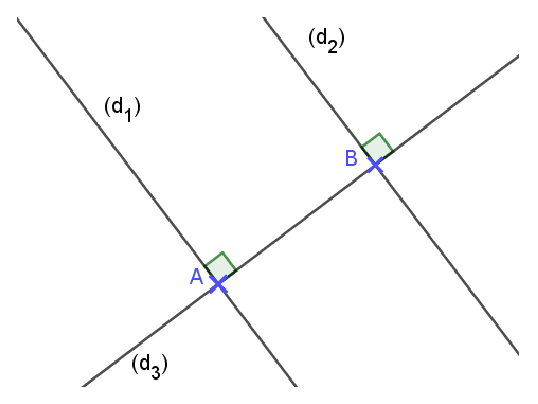
\includegraphics[scale=0.8]{Situation1.eps} \hspace*{2cm}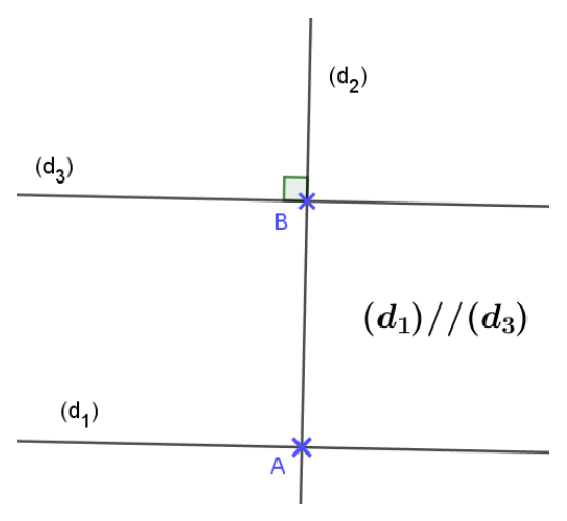
\includegraphics[scale=0.75]{Situation2.eps} \\

Les droites $(d_{1})$ et $(d_{2})$  sont . . . . . . . . . . . .  \hspace*{2cm}  Les droites $(d_{1})$ et $(d_{2})$  sont . . . . . . . . . . . .\\

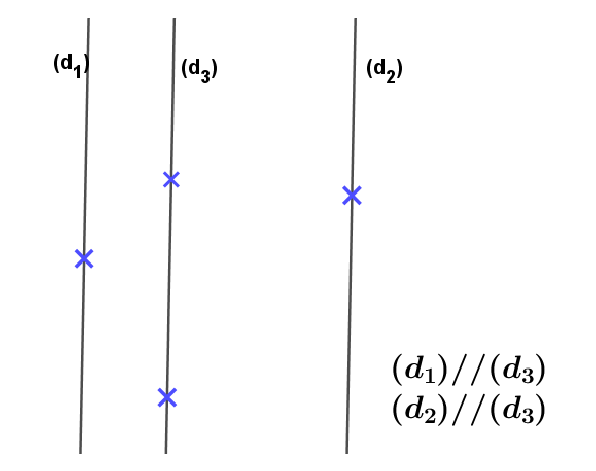
\includegraphics[scale=0.75]{Situation3.eps}  \\
Les droites $(d_{1})$ et $(d_{2})$  sont . . . . . . . . . . . . \\


\vspace*{1cm}

$\rightarrow$ \textbf{Distance, milieu et codages}\\

\vspace*{0.5cm}

\exo \\ Compléter la définition d'une longueur. \\

La longueur du segment [AB] se note . . . . \\

\exo \\ Compléter la définition d'un milieu d'un segment. \\

Le milieu d'un segment est le . . . . . . . . . qui appartient au segment et qui est à égale . . . . . . . . . . . . . . .  de ses extrémités.\\

\exo \\ Compléter la propriété du milieu d'un segment. \\

Si I est le milieu du segment [AB] alors $AI = .... = \dfrac{AB}{....}$\\


\exo \\ Placer les points A, B, C, D et E sur la figure suivante sachant que : \\
-  E est le milieu du segment [BC], \\
-  (AC) $\perp$  (BC) \\
-  AD = BD \\

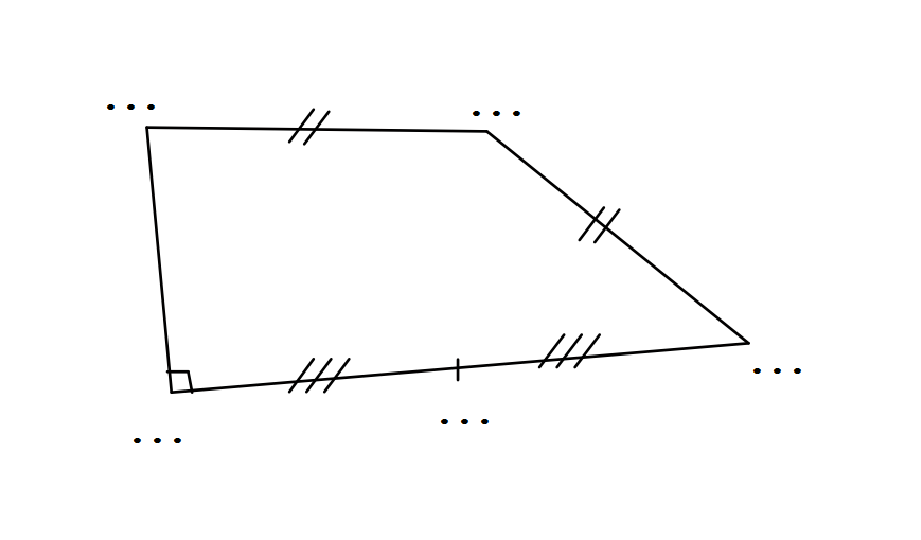
\includegraphics[scale=0.9]{distance2.eps} \\


\vspace*{1cm}

$\rightarrow$ \textbf{Les cercles}\\

\vspace*{0.5cm}


\exo \\ Parmi les phrases suivantes, quelles sont celles  qui désignent avec précision le cercle rouge dans la figure ci-dessous.\\


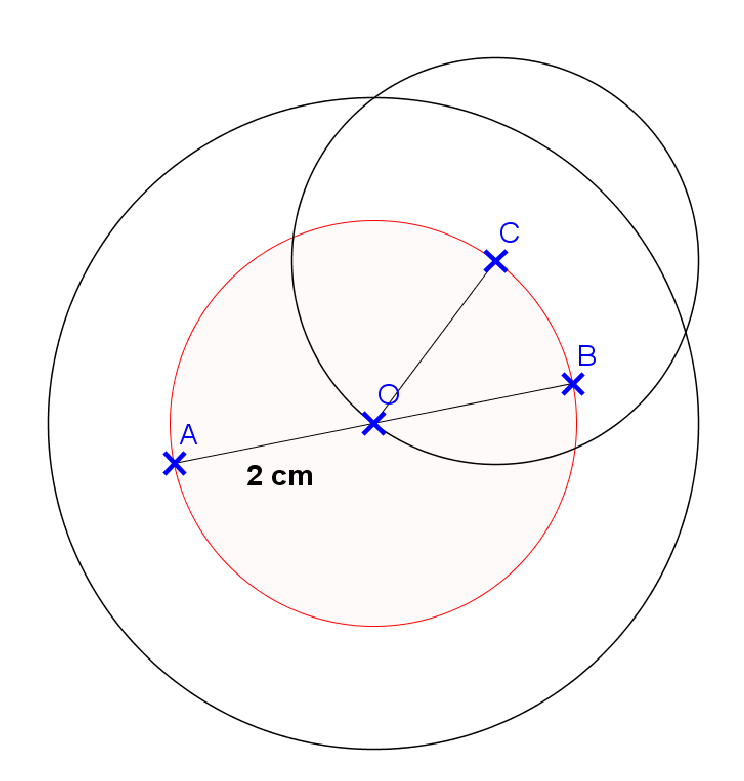
\includegraphics[scale=0.9]{cercle3.eps} \\

\initqa \qa Le cercle de centre O.\\

\qa Le cercle de rayon 2 cm.\\

 \qa Le cercle de centre O et de rayon 2 cm.\\

\qa Le cercle de diamètre [AB].\\

\qa Le cercle du rayon [OC].\\

Réponse : . . . . . . . . . . . . . . . . . . . . . . . . . . . .\\


\exo \\ Compléter la définition d'un rayon d'un cercle.\\

Un rayon est un . . . . . . . . qui a pour extrémités le . . . . . . . . . . . du cercle et un point du cercle.\\


\exo \\ Compléter la définition d'une corde d'un cercle.\\

Une corde est un . . . . . . . . . . joignant . . . points du cercle.\\


\exo \\ Compléter la définition d'un diamètre d'un cercle.\\

Un diamètre d'un cercle est une . . . . . . . passant par le . . . . . . du cercle. Sa longueur est égale au . . . . . . de celle du rayon.\\



\vspace*{1cm}

$\rightarrow$ \textbf{Les triangles}\\

\vspace*{0.5cm}




\exo \\ Compléter la définition d'un triangle rectangle.\\ 

Un triangle rectangle est un triangle qui possède . . . . côtés . . . . . . . . . . . . . . . . .\\

\exo \\ Compléter la définition d'un triangle isocèle.\\ 

Un triangle isocèle est un triangle qui possède . . . . . côtés de . . . . . . . . .longueurs.\\



\exo \\ Compléter la définition d'un triangle équilatéral.\\ 

Un triangle équilatéral est un triangle qui possède . . . . . côtés de . . . . . . . . .longueurs.\\


\exo \\ Compléter les pointillés par les mots : \textit{sommet(s)},  \textit{côté(s)},  \textit{opposé}.\\

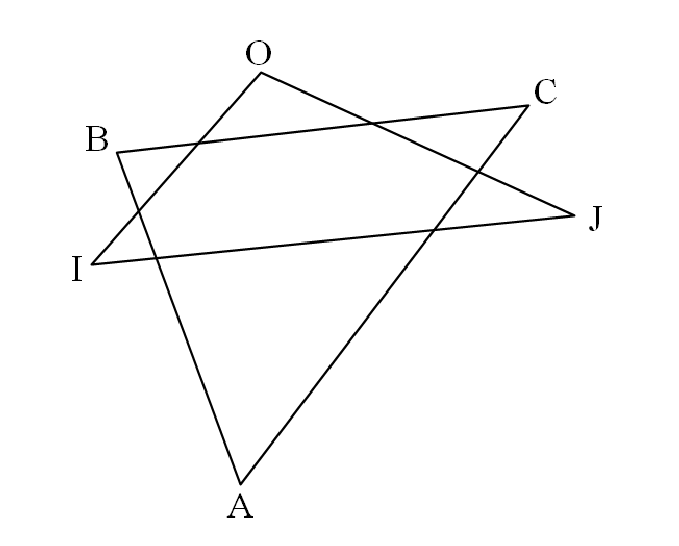
\includegraphics[scale=1]{triangle1.eps} \\

		\initqa \qa I, O et J sont les trois ...................... du triangle OIJ.\\
		
		\qa [IO], [OJ] et [IJ] sont les trois ...................... du triangle OIJ.\\
		
		\qa O est le ...................... ...................... au coté [IJ].\\
		
		\qa [OI] est le ...................... ...................... au sommet J.\\



\exo \\ Compléter les pointillés par les mots : \textit{sommet(s)},  \textit{côté(s)}, \textit{triangle}, \textit{opposé}.\\


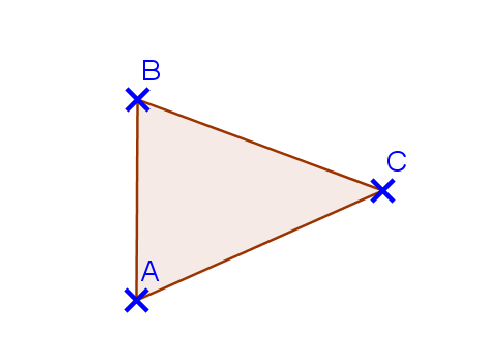
\includegraphics[scale=1]{triangle11.eps} \\

\initqa \qa ABC est un . . . . . . . .\\

\qa [AB] est un . . . . . . . . .\\

\qa Le point C est un . . . . . . . .\\

\qa [BC] est le . . . . . . . . \hspace*{0.4cm} . . . . . . . .  au . . . . . . . . A\\

\qa B est le . . . . . . . . \hspace*{0.4cm} . . . . . . . .  au . . . . . . . . [AC]\\
\vspace*{0.5cm}

\begin{center}
{\Large \textbf{Niveau 2 :}}
\end{center}

\vspace*{1cm}

$\rightarrow$ \textbf{Notations et vocabulaire}\\

\vspace*{0.5cm}

\exo \\ Compléter la définition d'une droite. \\

Une droite est une ligne droite . . . . . . . . . . . des deux côtés.\\



\exo \\ Compléter la définition d'une demi-droite. \\

Une demi-droite est une ligne droite . . . . . . . .  d'un côté par un point qu'on appelle . . . . . . . . . . . . . et . . . . . . . . . . . . de l'autre côté.\\


\exo \\ Indiquer le nom de chaque partie en violet sur chaque figure.\\

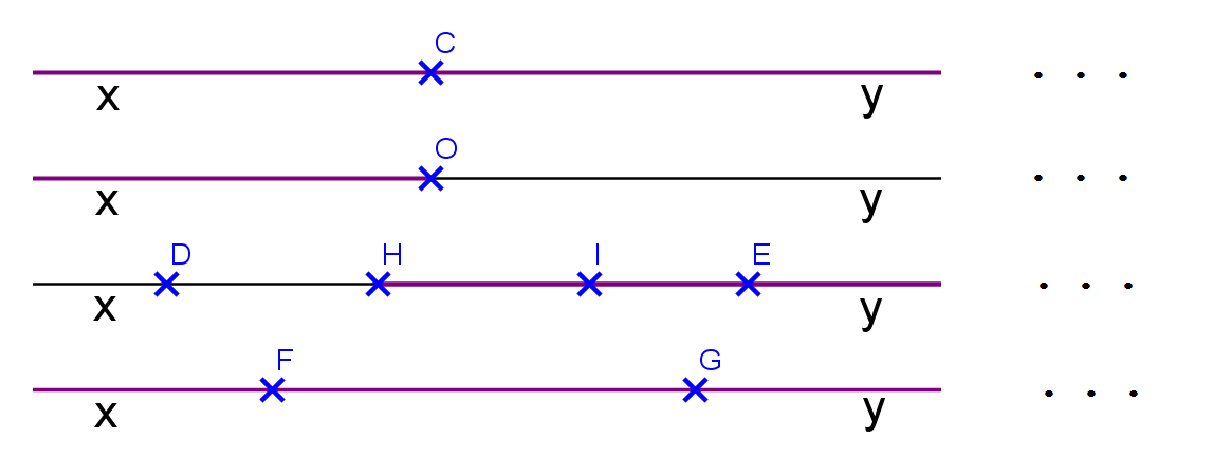
\includegraphics[scale=0.9]{notation4.eps} \\


\exo \\ Les points A, B et C appartiennent à la droite tracée ci-dessous.\\
Donner toutes les possibilités pour nommer cette droite.\\

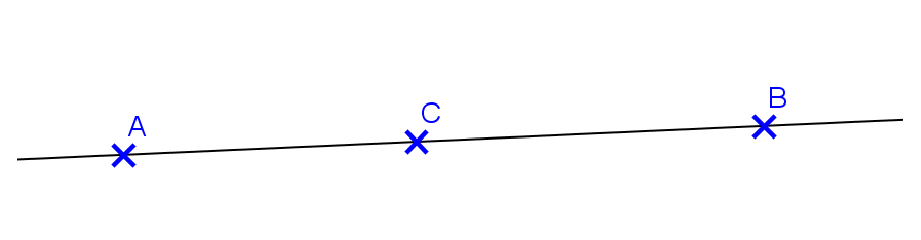
\includegraphics[scale=0.9]{notation9.eps} \\



\vspace*{1cm}

$\rightarrow$ \textbf{DROITES PARALLÈLES ET PERPENDICULAIRES : Savoir reconnaître des droites parallèles et perpendiculaires}\\

\vspace*{0.5cm}



\exo \\ Compléter les affirmations suivantes à l'aide des symboles suivants  : $\perp $ ou $\slash\slash$.\\

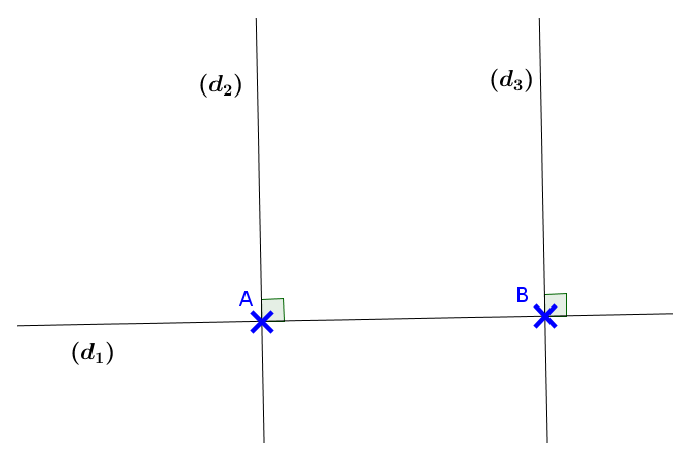
\includegraphics[scale=1]{defdroite1.eps} \\


\initqa \qa $(d_{3})$ . . . . $(d_{1})$\\

\qa $(d_{2})$ . . . . $(d_{1})$\\

\qa $(d_{2})$ . . . . $(d_{3})$\\




\exo \\ ABCD et GHEJ sont des carrés. Les droites ci-dessous sont-elles perpendiculaires ? Compléter à l'aide du symbole perpendiculaire.\\

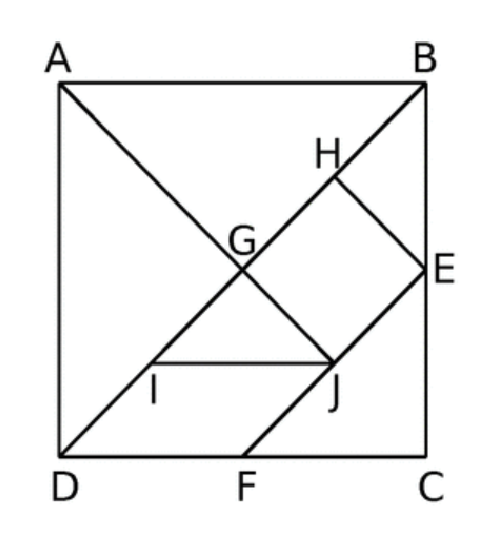
\includegraphics[scale=0.8]{defdroite8.eps} \\


\initqa \qa (AB) . . . (IJ)\\

\qa (HG) . . . (GJ)\\

\qa (BE) . . . (IJ)\\

\qa (DF) . . . (BG)\\

\qa (JE) . . . (AG)\\

\qa (AB) . . . (HE)\\



\exo \\ ABCD et GHEJ sont des carrés. Les droites ci-dessous sont-elles parallèles ? Compléter à l'aide du symbole parallèle.\\

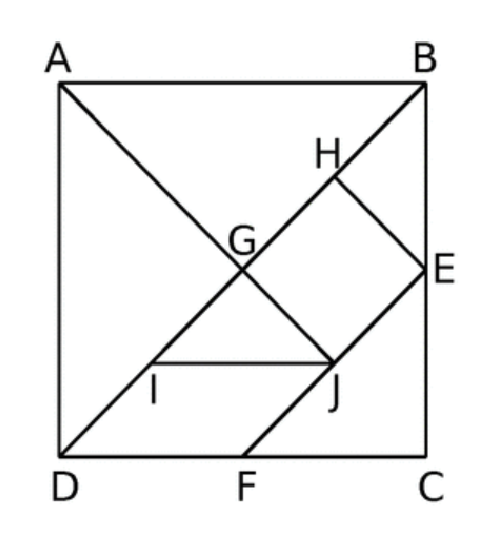
\includegraphics[scale=0.8]{defdroite8.eps} \\


\initqa \qa (BE) . . . (EJ)\\

\qa (IJ) . . . (FC)\\

\qa (JE) . . . (AD)\\

\qa (BD) . . . (AJ)\\

\qa (AB) . . . (IJ)\\

\qa (AJ) . . . (BC)\\

\vspace*{0.5cm}



\vspace*{1cm}

$\rightarrow$ \textbf{DROITES PARALLÈLES ET PERPENDICULAIRES : Savoir utiliser les propriétés des droites parallèles et perpendiculaires}\\

\vspace*{0.5cm}

\exo \\ En vous aidant de la figure ci-dessous, compléter à l'aide des symboles  $\perp $ ou $\slash\slash$.\\


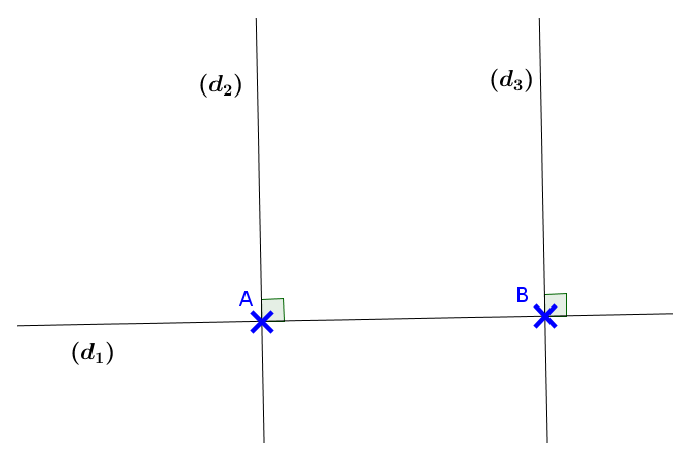
\includegraphics[scale=1]{defdroite1.eps} \\

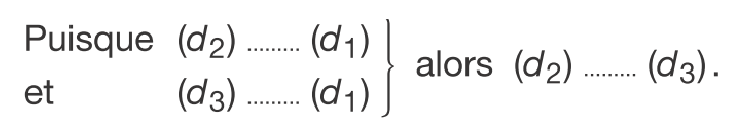
\includegraphics[scale=0.7]{propdroite1.eps} \\



\exo \\ En vous aidant des propriétés que vous avez apprises en classe, compléter les démonstrations suivantes à l'aide des symboles  $\perp $ ou $\slash\slash$.\\

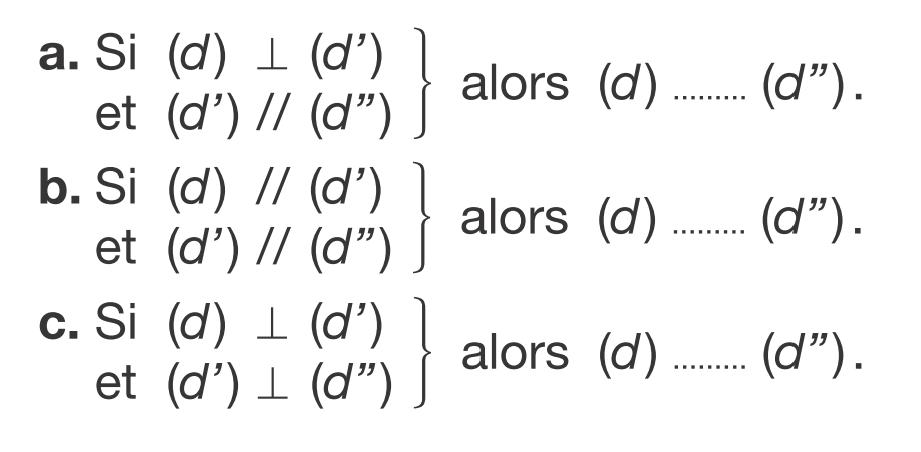
\includegraphics[scale=0.5]{propdroite2.eps} \\




\vspace*{1cm}

$\rightarrow$ \textbf{Distance, milieu et codages}\\

\vspace*{0.5cm}


\exo \\ Soit $(xy)$ une droite et deux points A et B appartenant à cette droite tels que : AB = 12 cm.\\
Soit C le point du segment [AB] tel que : AC = 7,8 cm.\\

 Calculer la distance BC.\\

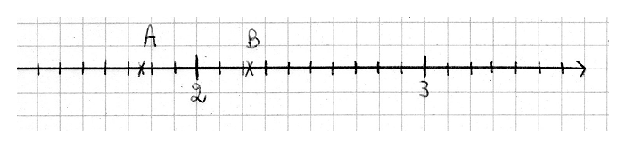
\includegraphics[scale=1]{droite.eps} \\

Calculs :\\
\reponse[2]\\

Phrase réponse :\\
\reponse[1]\\

\exo \\ Placer les points A, B, C, D, E et F sur la figure suivante sachant que : \\
-  E est le milieu du segment [FD], \\
-  (DC) $\perp$  (BC) \\
-  AF = DC \\

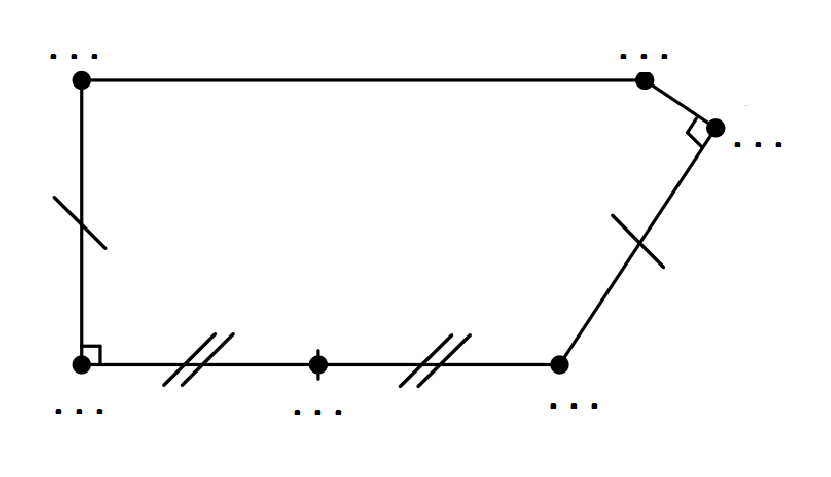
\includegraphics[scale=0.9]{distance3.eps} \\



\exo \\ Grâce aux codages de la figure, compléter les informations ci-dessous.\\

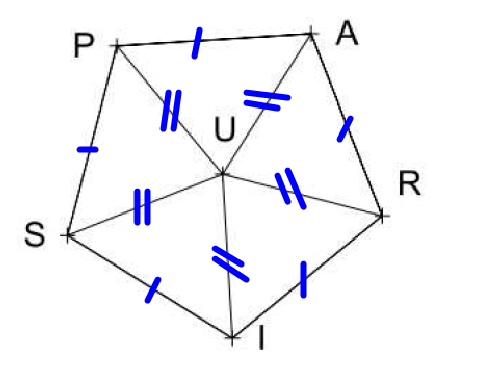
\includegraphics[scale=0.9]{distance4.eps} \\

- PA = . . . . =\\

- AU = . . . . =\\ 


\vspace*{1cm}

$\rightarrow$ \textbf{Les cercles}\\

\vspace*{0.5cm}


\exo \\ On donne la figure ci-dessous. Compléter les phrases suivantes par \textit{le} ou \textit{un}.\\

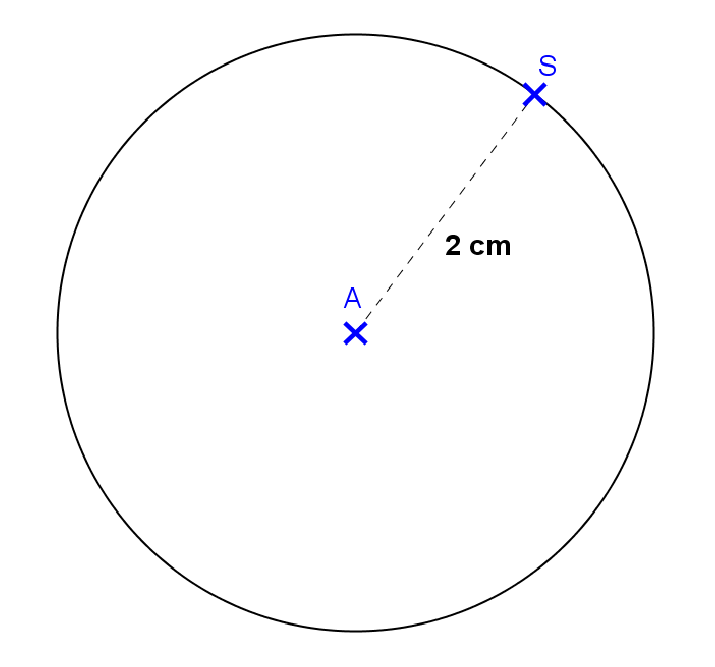
\includegraphics[scale=0.9]{cercle1.eps} \\

\initqa \qa Le segment [AS] est  . . . . rayon du cercle.\\

\qa 2 cm est . . . . rayon du cercle.\\

\qa La longueur AS est . . . . rayon du cercle.\\


\exo \\

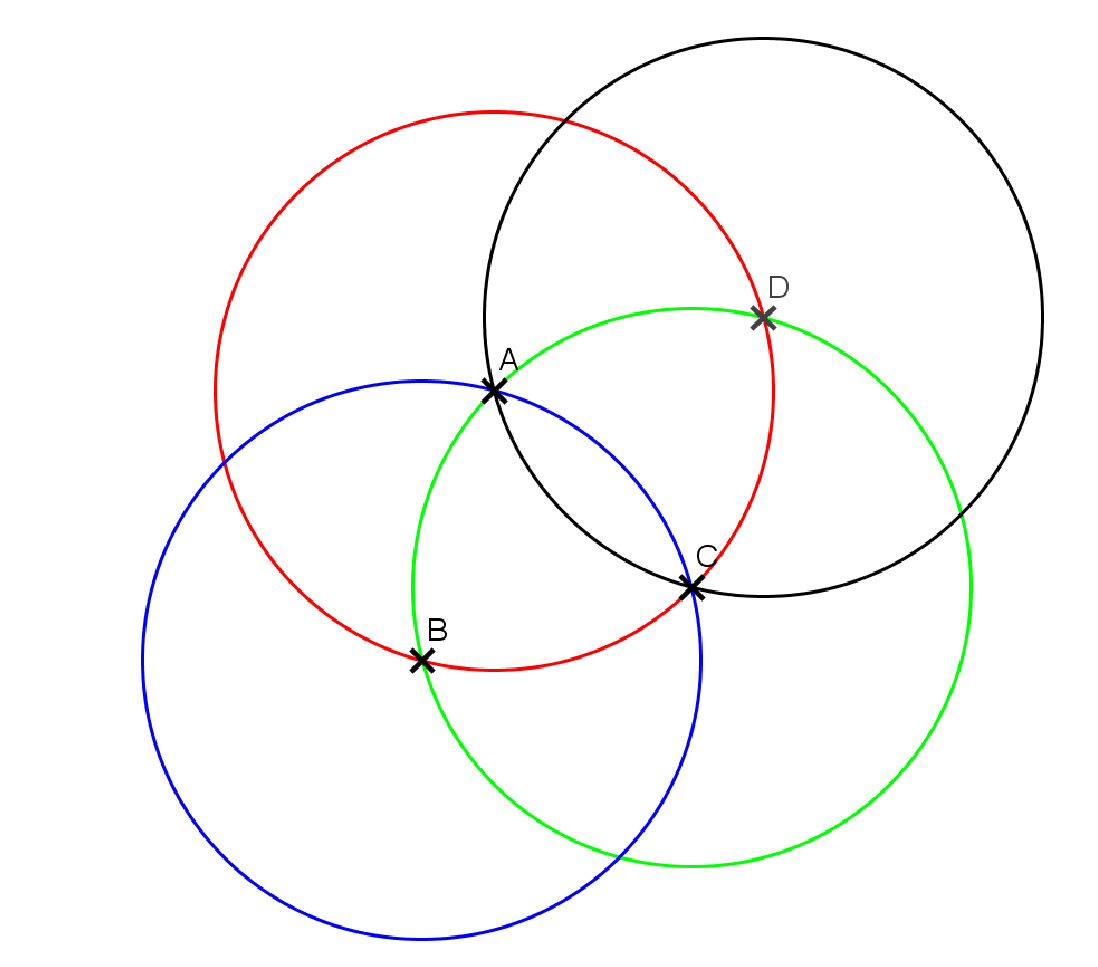
\includegraphics[scale=0.9]{cercle4.eps} \\

\initqa \qa Dans la figure ci-dessus, indiquer la couleur du cercle de centre A et qui passe par le point B.\\
\reponse[2]\\

\qa L'un des 4 cercles passe-t-il à la fois par les 4 points A, B , C et D ? Si oui, indiquer sa couleur.\\
\reponse[2]\\

\qa Quelle est la couleur du cercle qui passe à la fois par les points A, B et D ? Quel est son rayon ?\\
\reponse[2]\\

\qa Pour deux de ces cercles, le segment [AB] est un rayon. Indiquer leur couleur.\\
\reponse[2]\\


\vspace*{1cm}

$\rightarrow$ \textbf{Les triangles}\\

\vspace*{0.5cm}

\exo \\ Compléter les pointillés par les points et segments qui conviennent.\\

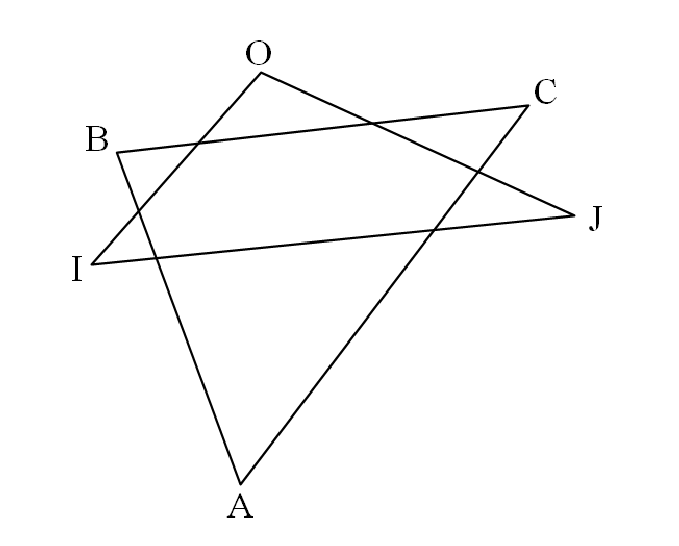
\includegraphics[scale=1]{triangle1.eps} \\


		\initqa \qa . . . ,  . . . et  . . . sont les trois sommets du triangle ABC.\\
		
		\qa  . . . ,  . . . et  . . . sont les trois côtés du triangle ABC.\\
		
		\qa  . . . est le sommet opposé au côté [AB].\\
		
		\qa  . . . est le côté opposé au sommet A.\\

\exo \\ Compléter les phrases suivantes à l'aide de la figure ci-dessous.\\

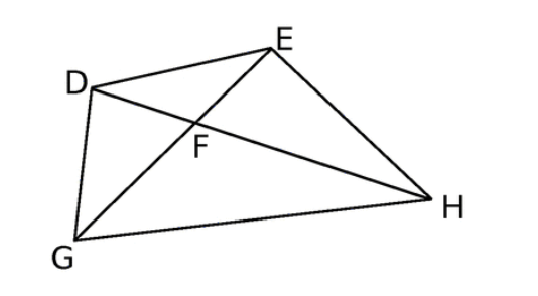
\includegraphics[scale=1]{triangle10.eps} \\

\initqa \qa Dans le triangle GFH, . . . . est le côté opposé au sommet F.\\

\qa Dans le triangle DHE, . . . .  est le sommet opposé au côté [EH] .\\

\qa Dans le triangle FEH, [FE] est le côté opposé au sommet . . . .\\

\qa Dans le triangle . . . . , E  est le sommet opposé au côté [GD] .\\




\exo \\ Combien y a-t-il de triangle sur l'image ci-dessous.\\



\includegraphics[scale=1]{triangle2.eps} \\

Réponse : . . . . . . . . . . .\\


\begin{center}
{\Large \textbf{Niveau 3 :}}
\end{center}

\vspace*{1cm}

$\rightarrow$ \textbf{Notations et vocabulaire}\\

\vspace*{0.5cm}



\exo \\ Que représente chacune des figures ci-dessous.\\

\begin{flushleft}
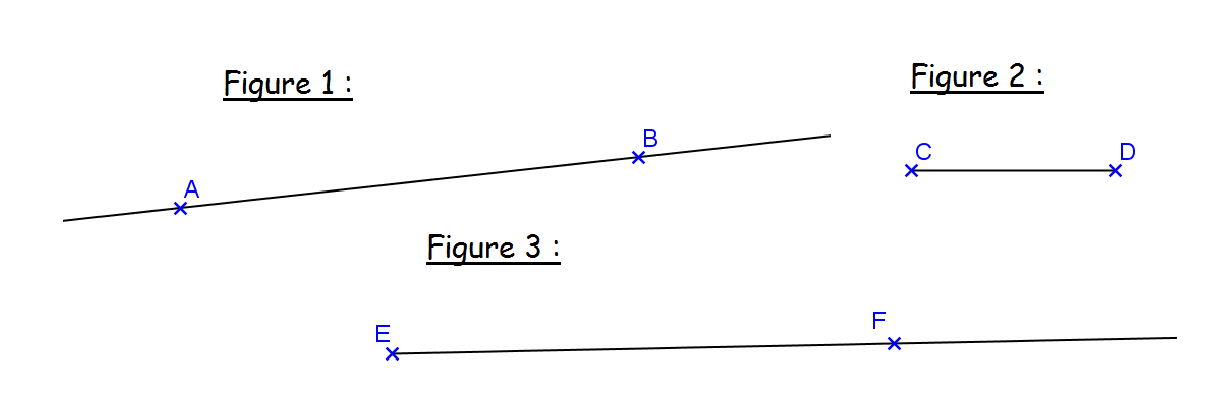
\includegraphics[scale=0.95]{notation1.eps} 
\end{flushleft}

\noindent Figure 1 : . . . . . . . . . . . \\
Figure 2 : . . . . . . . . . . . \\
Figure 3 : . . . . . . . . . . . \\


\exo \\ Vrai ou faux.\\

\initqa \qa "La droite (FA), c'est pareil que la droite (AF)" affirme Jean.\\
Est-ce exact ? . . . . . . . . . . .\\


\qa "Le segment [TS], c'est pareil que le segment [ST]" affirme Léa.\\
Est-ce exact ? . . . . . . . . . . .\\


\qa "La demi-droite [DO), c'est pareil que la demi-droite [OD)" affirme Pascal.\\
Est-ce exact ? . . . . . . . . . . .\\


\exo \\ Indiquer le nom de chaque partie en gras sur chaque figure.\\

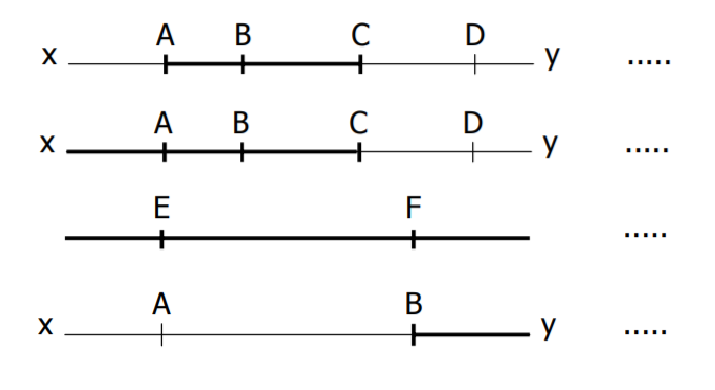
\includegraphics[scale=0.9]{notation5.eps} \\

\exo \\ Dans chaque écrire avec les notations mathématiques.\\

\initqa \qa Le segment d'extrémités E et F : . . . . . .\\

\qa La droite passant par les points K et L : . . . . . .\\

\qa La demi-droite d'origine R et qui passe par le point U : . . . . . .\\

\qa La demi-droite d'origine U et qui passe par le point R : . . . . . .\\

\vspace*{0.5cm}



\vspace*{1cm}

$\rightarrow$ \textbf{DROITES PARALLÈLES ET PERPENDICULAIRES : Savoir reconnaître des droites parallèles et perpendiculaires}\\

\vspace*{0.5cm}


\exo \\ En utilisant le quadrillage, compléter le tableau.\\


\begin{flushleft}
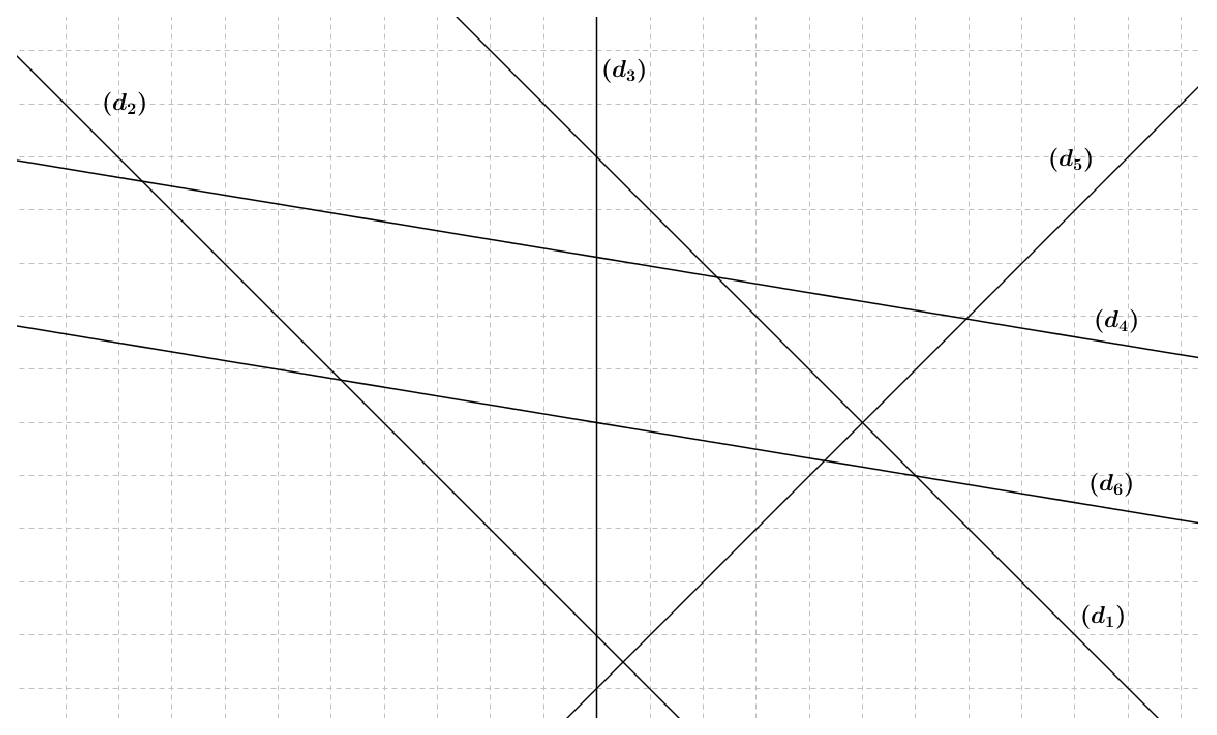
\includegraphics[scale=0.9]{defdroite6.eps} 
\end{flushleft}

\renewcommand\arraystretch{2.5}

\begin{tabular}{|p{8cm}|p{8cm}|}
\hline 
Droites parallèles & Droites perpendiculaires \\ 
\hline 
 & \\ 
\hline 
\end{tabular} 


\exo \\ A l'aide de la figure ci-dessous, répondre aux questions suivantes.\\

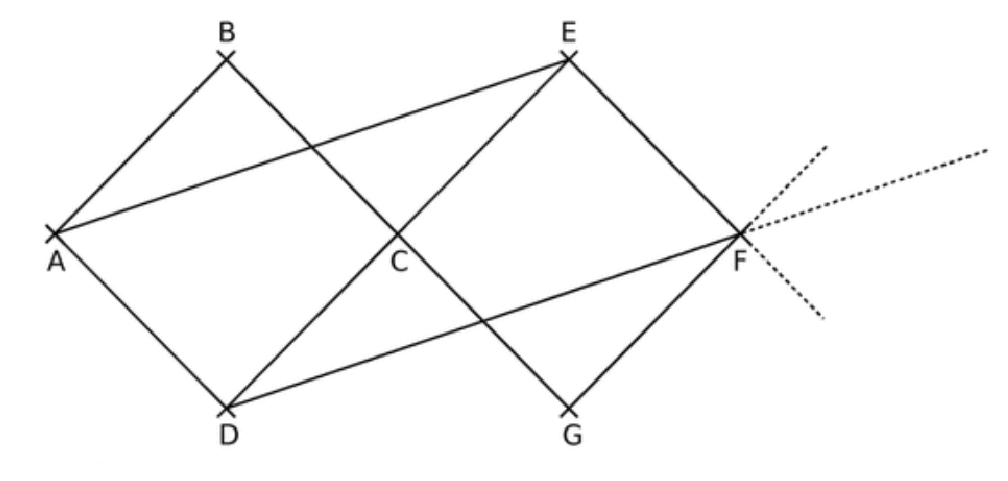
\includegraphics[scale=0.9]{defdroite7.eps} \\

\initqa \qa Quelle est la droite parallèle à (AD) passant par le point C ? . . . . . . . . . . . . . . . . . . . . . . . . . . . . . \\

\qa Quelle est la droite parallèle à (AE) passant par le point D ? . . . . . . . . . . . . . . . . . . . . . . . . . . . . . \\

\qa Quelle est la droite perpendiculaire à (CE) passant par le point D ? . . . . . . . . . . . . . . . . . . . . . . . . . . . . . \\


\qa Quelle est la droite perpendiculaire à (AB) passant par le point E ? . . . . . . . . . . . . . . . . . . . . . . . . . . . . . \\


\vspace*{1cm}

$\rightarrow$ \textbf{DROITES PARALLÈLES ET PERPENDICULAIRES : Savoir utiliser les propriétés des droites parallèles et perpendiculaires}\\

\vspace*{0.5cm}

\exo \\ Cliquer sur la bonne réponse. Il n'y a qu'une réponse possible par ligne.\\
\renewcommand{\arraystretch}{2}

\begin{tabular}{|p{6cm}|c|c|c|}
\hline 
On sait que : (AB) $\slash\slash$ (CD) et que  (AB) $\slash\slash$ (EF) alors ...  & (CD) $\slash\slash$ (EF) & (EF) $\perp$ (CD) & On ne peut rien dire \\ 
\hline 
On sait que : (d) $\slash\slash$ (d'),  (d'') $\perp$ (d') et que (d'') $\perp(\Delta)$  alors ... & (d) $\slash\slash (\Delta)$  & (d) $\perp (\Delta)$ & On ne peut rien dire \\ 
\hline 
On sait que :  (d) et (d') sont sécantes, (d'') $\perp$ (d') et que (d) $\slash\slash (\Delta)$ alors ... & (d'') $\perp (\Delta)$ &  $(\Delta)$ et (d'') sont sécantes & On ne peut rien dire \\ 
\hline 
\end{tabular} 

\exo \\ Dans le quadrilatère suivant, on sait qu'il y a 3 angles droits.\\

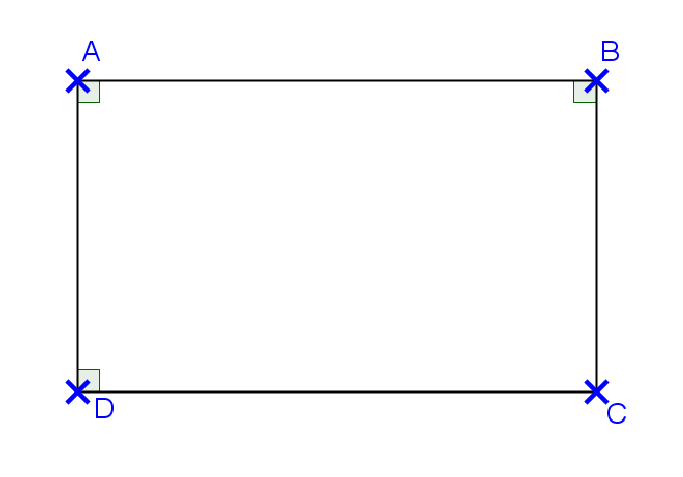
\includegraphics[scale=0.8]{propdroite3.eps} \\

 En vous aidant des propriétés que vous avez apprises en classe, compléter les démonstrations suivantes à l'aide des symboles  $\perp $ ou $\slash\slash$.\\
 
\initqa \qa

 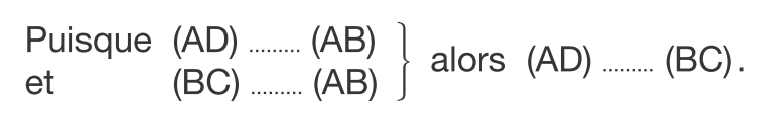
\includegraphics[scale=0.6]{propdroite3a.eps} \\

\qa 

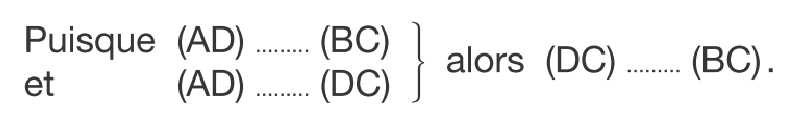
\includegraphics[scale=0.6]{propdroite3b.eps} \\

\exo \\ On considère la figure ci-contre.\\
On veut montrer que les droites $(d_{2})$ et $(d_{3})$ sont parallèles. \\
Pour cela compléter la démonstration ci-dessous.\\


\begin{flushleft}
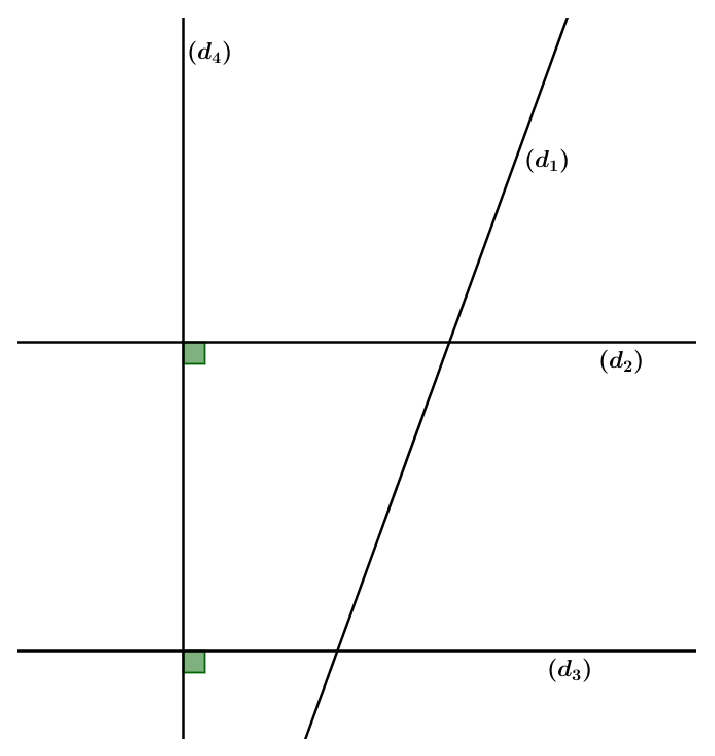
\includegraphics[scale=0.52]{propdroite4.eps} 
\end{flushleft}

\textbf{On sait que :}  $(d_{2}) ......... (d_{4})$  et  $(d_{3}) ......... (d_{4})$\\

\textbf{Or,} si deux droites sont . . . . . . . . . . . . . . . . . . à une même droite, alors elles sont . . . . . . . . . . . . . . . . . . entre elles.\\

\textbf{Donc,} $(d_{2}) ......... (d_{3})$\\


\vspace*{1cm}

$\rightarrow$ \textbf{Distance, milieu et codages}\\

\vspace*{0.5cm}




\exo \\ Dans la figure ci-dessous C est le milieu du segment [AB] et D est le milieu du segment [CB].\\
On suppose également que DC = 2,4 cm.\\

Calculer la longueur du segment [AB].\\

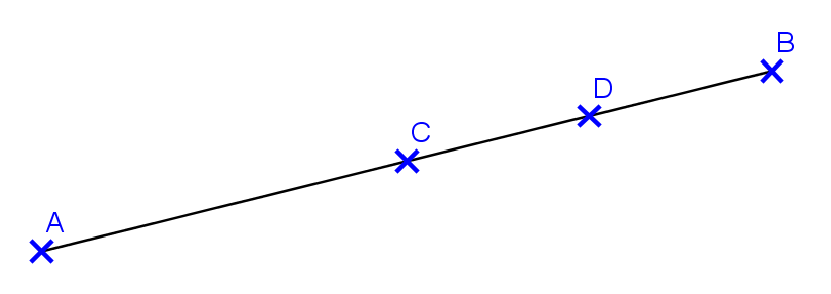
\includegraphics[scale=0.85]{distance1.eps} \\


Calculs : \\
\reponse[2]\\

Phrase réponse :\\
\reponse[1]\\





\exo \\ Soit $(xy)$ une droite et deux points A et B appartenant à cette droite tels que : AB = 12 cm.\\
Soit C le point du segment [AB] tel que : AC = 7,8 cm. Soit le point I, milieu du segment [AC]. 
\\

Calculer la distance IC.\\

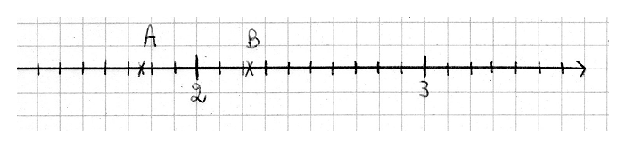
\includegraphics[scale=1]{droite.eps} \\

Calculs :\\
\reponse[2]\\

Phrase réponse :\\
\reponse[1]\\



\exo \\ Grâce aux codages de la figure, compléter les informations ci-dessous.\\

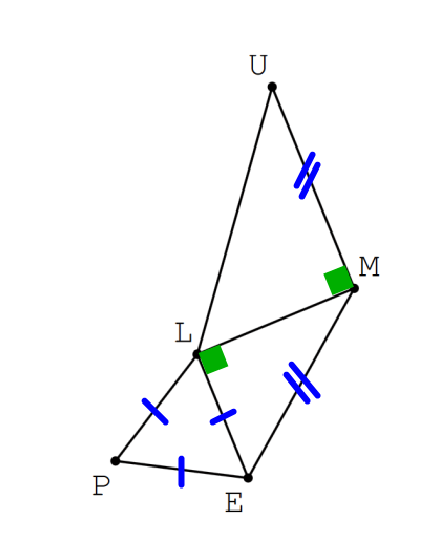
\includegraphics[scale=0.9]{distance5.eps} \\

- LE = . . . . =\\

- ME = . . . . =\\ 

- . . . $\perp$ . . .\\

- . . . $\perp$ . . .\\


\vspace*{1cm}

$\rightarrow$ \textbf{Les cercles}\\

\vspace*{0.5cm}





\exo \\ On donne la figure ci-dessous. Compléter les phrases suivantes en utilisant les mots : \textit{rayon}, \textit{diamètre}, \textit{corde}, \textit{milieu} et \textit{centre}.\\

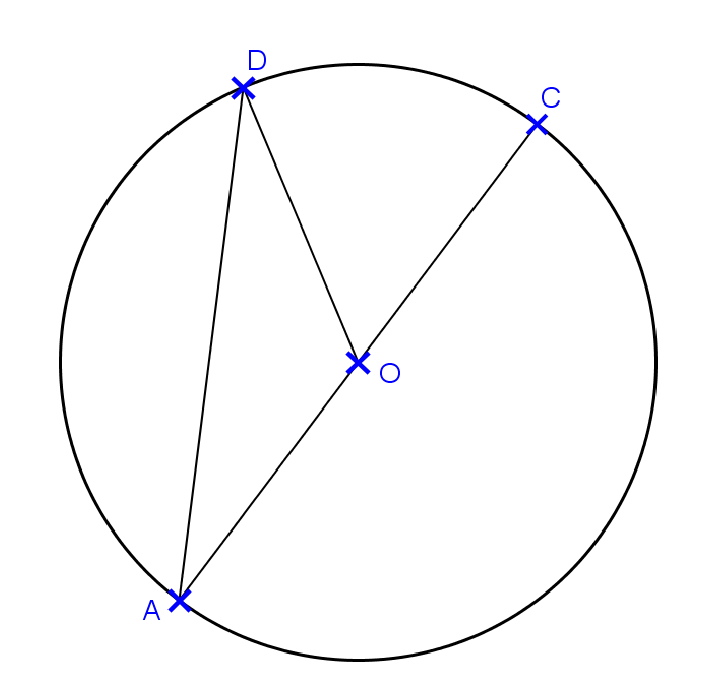
\includegraphics[scale=0.9]{cercle2.eps} \\


\initqa \qa Le point O est le . . . .  du cercle. C'est aussi le . . . . . . du . . . . . . . . [AC].\\


\qa [OA] , [OC] , [OD] sont des . . . . . . . . . . du cercle.\\

\qa [AD] et [AC] sont des . . . . . . . . . du cercle.\\

\vspace*{1cm}

$\rightarrow$ \textbf{Les triangles}\\

\vspace*{0.5cm}


\exo \\ 

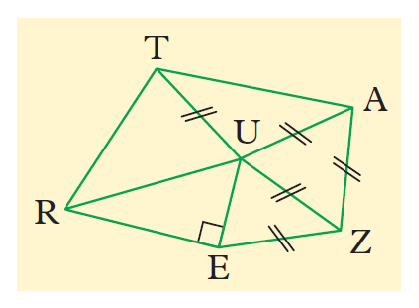
\includegraphics[scale=0.9]{triangle3.eps} \\

En observant le codage de la figure ci-dessus, citer :\\

\initqa \qa un triangle rectangle : . . . . . . . . . . .\\

\qa un triangle équilatéral : . . . . . . . . . . .\\

\qa deux triangles isocèles qui ne sont pas équilatéraux : . . . . . . . . . . .\\

\qa un triangle qui ne paraît ni isocèle ni rectangle : . . . . . . . . . . .\\



\exo \\ 

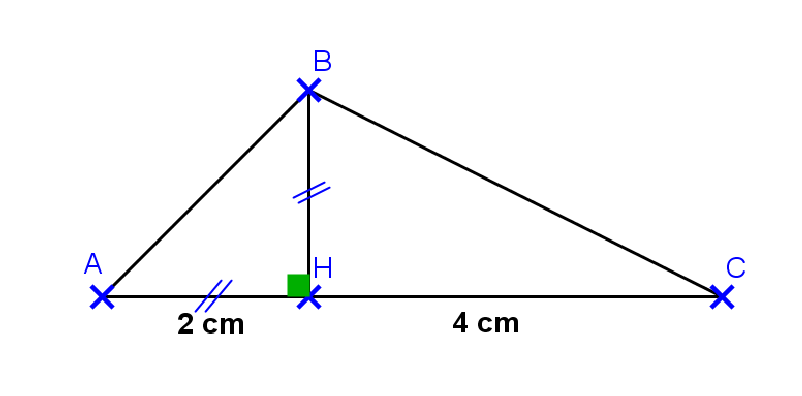
\includegraphics[scale=0.9]{triangle4.eps} \\

En observant le codage de la figure ci-dessus, citer :\\

\initqa \qa un triangle isocèle : . . . . . . . . . . .\\


\qa deux triangles rectangles : . . . . . . . . . . .\\

\qa un triangle rectangle et isocèle : . . . . . . . . . . . . .\\

\qa un triangle qui n'est ni isocèle ni rectangle : . . . . . . . . . . .\\




\exo \\ Classer les triangles ci-dessous dans le tableau par rapport à leur propriété.\\

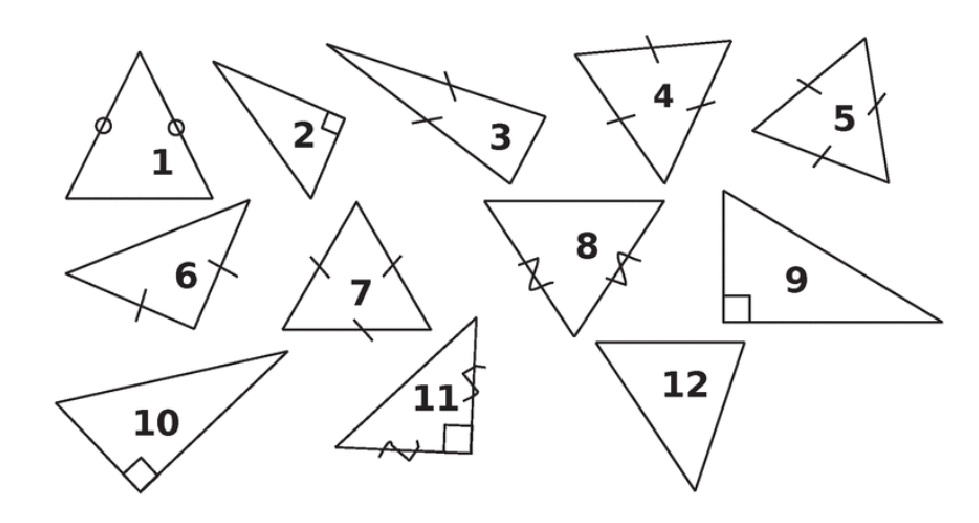
\includegraphics[scale=0.9]{triangle9.eps} \\

\begin{tabular}{|c|p{9cm}|}
\hline 
\textbf{Les triangles quelconques :} & . . . . . . . . . . . . . . . . . . . . . .\\ 
\hline 
\textbf{Les triangles rectangles :} & . . . . . . . . . . . . . . . . . . . . . .\\ 
\hline 
\textbf{Les triangles isocèles qui ne sont pas équilatéraux :} & . . . . . . . . . . . . . . . . . . . . . . \\ 
\hline 
\textbf{Les triangles équilatéraux :}& . . . . . . . . . . . . . . . . . . . . . . \\ 
\hline 
\end{tabular} 


\begin{center}
{\Large \textbf{Niveau 4:}}
\end{center}

\vspace*{1cm}

$\rightarrow$ \textbf{Notations et vocabulaire}\\

\vspace*{0.5cm}



\exo \\ Compléter la définition de points alignés. \\

Des points sont alignés lorsqu'ils appartiennent à une même . . . . . . . . . . . . .\\


\exo \\ Lister tous les segments, droites et demi-droites que vous voyez en utilisant les bonnes notations.\\

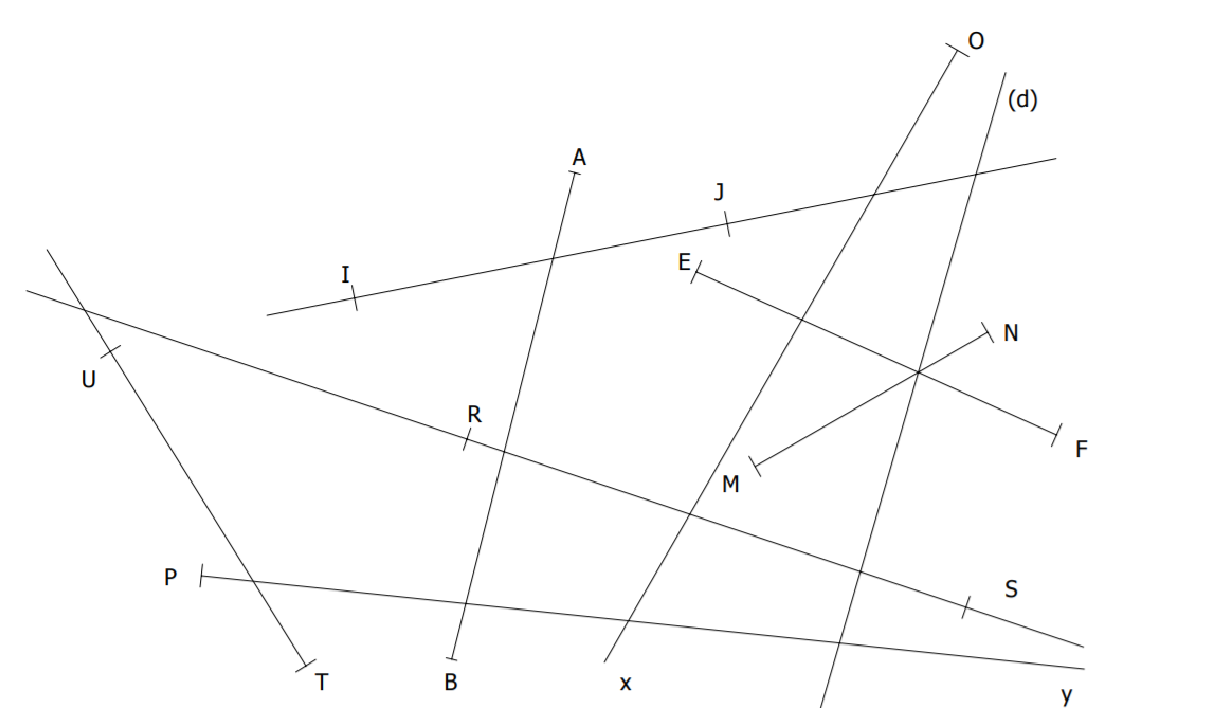
\includegraphics[scale=0.9]{notation6.eps} \\

\begin{tabular}{|c|p{9cm}|}
\hline 
 Les segments : &  \\ 
\hline 
Les droites :  &  \\ 
\hline 
Les demi-droites :  &  \\ 
\hline 
\end{tabular} 



\exo \\  Compléter avec les symboles $\in $ ou $\notin$.\\

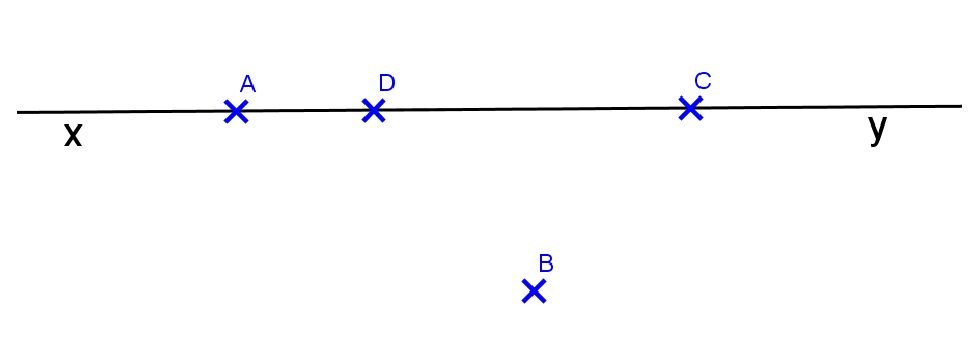
\includegraphics[scale=0.9]{notation7.eps} \\


\initqa \qa B . . . . . (AC)\\

\qa A . . . . . (AC)\\

\qa A . . . . . [DC]\\

\qa D . . . . . (yx)\\

\qa C . . . . . [DA)\\

\qa A . . . . . [Dx)\\




\vspace*{1cm}

$\rightarrow$ \textbf{DROITES PARALLÈLES ET PERPENDICULAIRES : Savoir reconnaître des droites parallèles et perpendiculaires}\\

\vspace*{0.5cm}


\exo \\ Compléter le texte suivant pour qu'il corresponde à la figure ci-dessous.\\

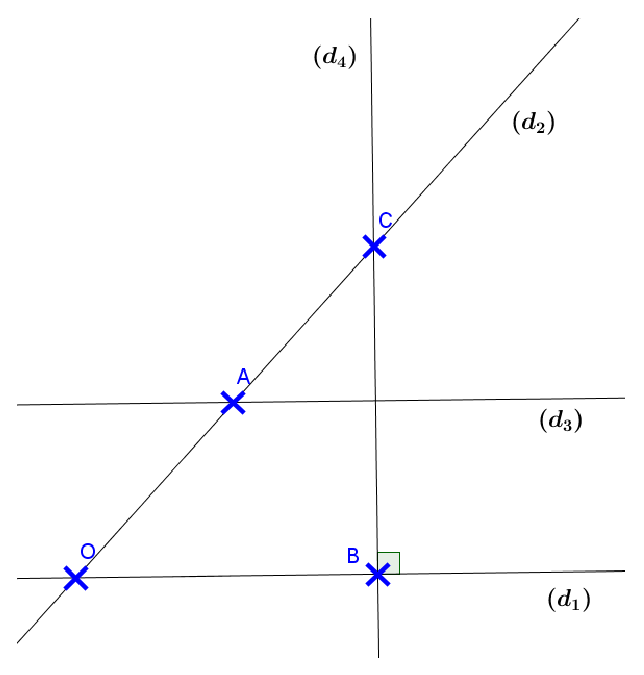
\includegraphics[scale=1]{defdroite2.eps} \\

Théa a tracé deux droites $(d_{1})$ et $(d_{2})$ . . . . . . . . . . . en 0.\\
Elle place ensuite une point  . . . . sur $(d_{1})$ et un point . . . . sur $(d_{2})$.\\
Elle construit la droite $(d_{3})$ . . . . . . . . . . . . . . . . . . à la droite $(d_{1})$ passant par A et la droite $(d_{4})$ . . . . . . . . . . . . . . . . . . à la droite $(d_{1})$ passant par B.\\
Les droites $(d_{2})$ et $(d_{4})$ sont . . . . . . . . . . . en . . . .\\


\exo \\ Compléter les phrases suivantes en vous aidant de la figure ci-dessous.\\

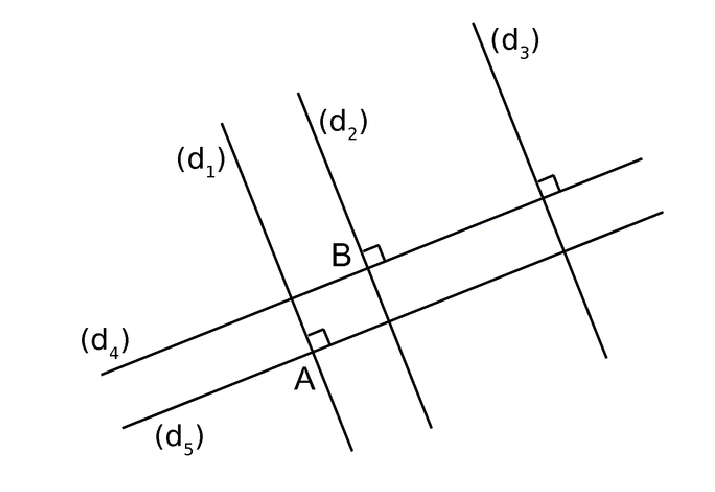
\includegraphics[scale=0.9]{defdroite5.eps} \\

\initqa \qa La droite $(d_{5})$ est . . . . . . . . . . . . . . . . . . . . à la droite  $(d_{1})$ passant par le point . . . .\\

\qa Les droites $(d_{4})$ et . . . . . . sont . . . . . . . . . . . . . . en B.\\

\qa $(d_{4})$ est . . . . . . . . . . . . . . à la droite $(d_{2})$ et à la droite $(d_{3})$.\\


\vspace*{1cm}

$\rightarrow$ \textbf{DROITES PARALLÈLES ET PERPENDICULAIRES : Savoir utiliser les propriétés des droites parallèles et perpendiculaires}\\

\vspace*{0.5cm}





\exo \\ Dans la figure ci-dessous, AEFB est un quadrilatère.\\
On souhaite démontrer les droites (AE) et (FB) sont parallèles.\\
A vous de compléter la démonstration.\\

\begin{center}
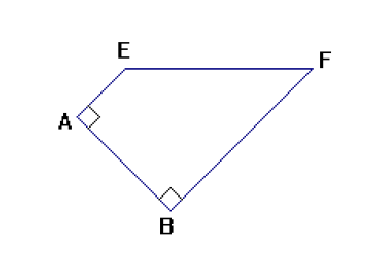
\includegraphics[scale=1]{interro2.eps} 
\end{center}



\textbf{On sait que :} . . . .  $\perp$ . . . .  et  . . . . $\perp$ . . . .\\

\textbf{Or,} si deux droites sont . . . . . . . . . . . . . . . . . . à une même droite, alors elles sont . . . . . . . . . . . . . . . . . . entre elles.\\

\textbf{Donc,} . . .  \hspace*{0.4cm}   . . . \hspace*{0.4cm}   . . . \\



\exo{2} \\ Dans la figure ci-contre, ABCD est un carré. \\
Les droites (DE) et (BF) sont parallèles. \\
On souhaite démontrer que les droites (AG) et (BF) sont perpendiculaires.\\
A vous de compléter la démonstration.\\

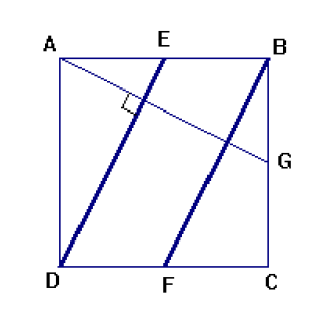
\includegraphics[scale=1]{interro3.eps} \\



\textbf{On sait que :}  . . . .  $\perp$ . . . .  et  . . . . $\slash\slash$ . . . .\\

\textbf{Or,} Si deux droites sont . . . . . . . . . . . . . . . . . et si une troisième droite est . . . . . . . . . . . . . . . . . à l'une, alors elle est . . . . . . . . . . . . . . à l'autre.\\

\textbf{Donc,} . . . . $\perp$ . . . . \\


\exo \\ On souhaite démontrer que les droites $(d_{1})$ et $(d_{1})$ sont parallèles.\\
A vous de compléter la démonstration.\\

\includegraphics[scale=1]{situation3.eps} \\


\textbf{On sait que :}  . . . .  $\slash\slash$ . . . .  et  . . . . $\slash\slash$ . . . .\\

\textbf{Or,} Si deux droites sont . . . . . . . . . . . . . . . . . à une même droite  alors elles sont . . . . . . . . . . . . . . entre elles.\\

\textbf{Donc,} . . . . $\slash\slash$ . . . . \\

\vspace*{1cm}

$\rightarrow$ \textbf{Distance, milieu et codages}\\

\vspace*{0.5cm}


\exo \\ Compléter la définition d'une médiatrice. \\

La médiatrice d'un segment est la . . . . . . qui passe par le . . . . . . . . du segment et qui lui est . . . . . . . . . . . . . . . . . . . . .\\

\exo \\

Parmi les phrases suivantes, indiquer celle qui correspond à la définition de la médiatrice du segment [AB]:\\

\initqa 
\qa La droite qui passe par le milieu du segment [AB];\\
\qa  La droite perpendiculaire au segment [AB];\\
\qa La droite qui passe par A;\\
\qa La droite qui passe par le milieu de [AB] et qui est perpendiculaire au segment [AB].\\ 

Réponse : . . . . . . . \\

\exo \\ Vrai ou faux\\

\initqa \qa Si $IA = IB$, alors I est le milieu de [AB] : . . . . . .\\

\qa Si $I \in (AB)$ et $AB = 2 \times IB$, alors I est le milieu de [AB] : . . . . . .\\

\exo \\ Dans quels cas, la droite (d) est-elle la médiatrice du segment [AB]?\\ Justifier votre réponse réponse.\\

\begin{flushleft}
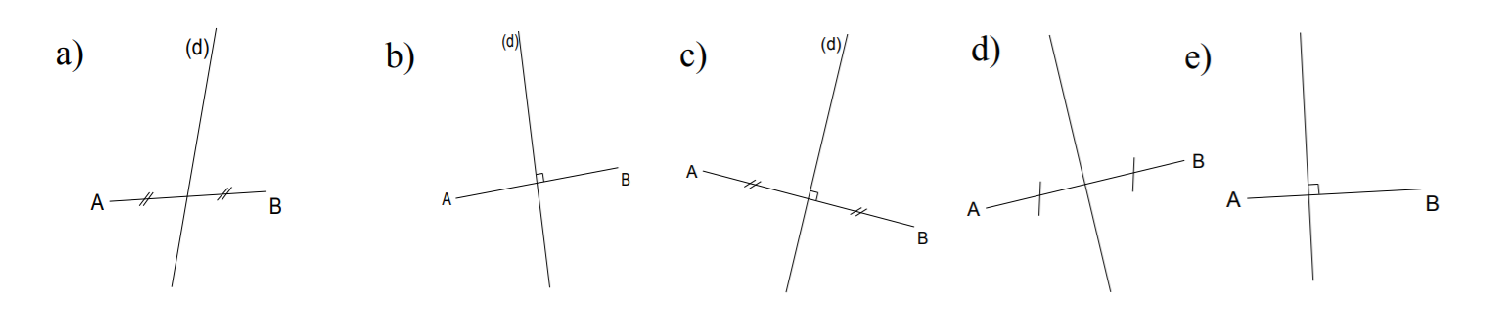
\includegraphics[scale=0.8]{exomediatrice1.eps} 
\end{flushleft}

Réponse : On peut dire que la droite ($d$) dans le cas . . . . est la . . . . . . . médiatrice du segment [AB] car elle passe par son . . . . . . . . . .  et lui est . . . . . . . . . . . . . . . . . . . .\\


\vspace*{1cm}

$\rightarrow$ \textbf{Les cercles}\\

\vspace*{0.5cm}


\exo{1} Compléter les phrases suivantes à l'aide du vocabulaire relatif au cercle :

\bmul{2}

Le point O est . . . . . . . . . . . . . . . . . . . . . . du cercle.\\

$[AB]$ est . . . . . . . . . . . . . . . . . . . . . . du cercle.\\

Le point O est . . . . . . . . . . . . . . . .  du segment $[AM]$.\\

 $[AM]$ est . . . . . . . . . . . . . . . . . . . . . . du cercle.\\
  On a  $AM = 2 \times .....$\\

\columnbreak


\begin{flushright}
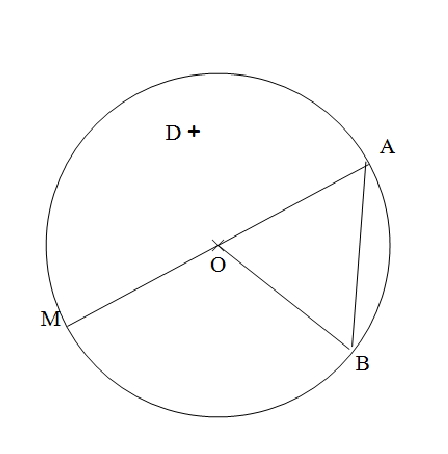
\includegraphics[scale=0.75]{exointerrocercle3.eps} 
\end{flushright}



\emul


\vspace*{1cm}

$\rightarrow$ \textbf{Les triangles}\\

\vspace*{0.5cm}


\exo \\ Vrai ou faux.\\

\initqa \qa Un triangle équilatéral est toujours isocèle : . . . .\\

\qa Un triangle isocèle est toujours équilatéral : . . . .\\

\qa Un triangle équilatéral peut être rectangle : . . . .\\

\qa Un triangle isocèle peut être rectangle : . . . .\\


\exo \\ Quelle est la nature du triangle GHI? Justifier votre réponse avec le cours.\\


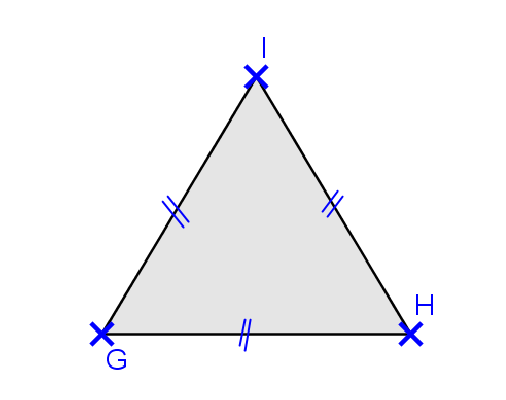
\includegraphics[scale=1]{triangle6.eps} \\

Le triangle GHI possède . . . . . . . . . . . . . . . . . . . . . . . donc c'est un triangle . . . . . . . . . .\\




\exo \\ Quelle est la nature du triangle EDF? Justifier votre réponse avec le cours.\\


\includegraphics[scale=1]{triangle7.eps} \\

Le triangle EDF possède . . . . . . . . . . . . . . . . . . . . . . . donc c'est un triangle . . . . . . . . . . en . . .\\

\exo \\ Quelle est la nature du triangle GHI? Justifier votre réponse avec le cours.\\


\includegraphics[scale=1]{triangle8.eps} \\

Le triangle JLK possède . . . . . . . . . . . . . . . . . . . . . . . donc c'est un triangle . . . . . . . . . . en . . .\\


\begin{center}
{\Large \textbf{Niveau 5 :}}
\end{center}

\vspace*{1cm}

$\rightarrow$ \textbf{Notations et vocabulaire}\\

\vspace*{0.5cm}

\exo \\ Compléter avec les symboles $\in $ ou $\notin$.\\

\bmul{2}

\includegraphics[scale=1]{exointerro8.eps} 

\columnbreak

\bmul{2}

B . . . [AH)\\

F  . . . (DE)\\

G . . . [FG] \\


\columnbreak
C . . . [AE]\\

H  . . . [BA)\\

A . . .  [HB)\\

\emul


\emul



\exo \\ Compléter avec les symboles $\in $ ou $\notin$.\\

\includegraphics[scale=0.9]{notation8.eps} \\


\initqa \qa E . . . . . (AB)\\

\qa D . . . . . [CA)\\

\qa E . . . . . [AB]\\

\qa B . . . . . (AC)\\

\qa B . . . . . [AB]\\

\qa D . . . . . [AC)\\


\exo \\ Vrai ou Faux.\\


\initqa \qa Si C $\in$ (AB) alors A $\in$ (BC). \\
Réponse : . . . . . . .\\

\qa Si E $\in$ [DF] alors D $\in$ [EF]. \\
Réponse : . . . . . . .\\

\qa Si C $\in$ [AB) mais C $\notin$ [AB] alors A $\in$ [CB). \\
Réponse : . . . . . . .\\

\qa Si C $\in$ [BA) et D $\in$ [AC) alors B $\in$ [DA). \\
Réponse : . . . . . . .\\


\vspace*{1cm}

$\rightarrow$ \textbf{DROITES PARALLÈLES ET PERPENDICULAIRES : Savoir reconnaître des droites parallèles et perpendiculaires}\\

\vspace*{0.5cm}


\exo \\ En observant les figures ci-dessous, compléter les phrases en utilisant les mots proposés.\\

\fbox{perpendiculaire(s)} \hspace*{1.5cm} \fbox{angle droit} \hspace*{1.5cm} \fbox{parallèle(s)} \hspace*{1.5cm} \fbox{sécante(s)} \\

\fbox{une parallèle} \hspace*{1.5cm} \fbox{la perpendiculaire} \hspace*{1.5cm} \fbox{une perpendiculaire} \hspace*{1.5cm} \fbox{la parallèle}\\

\includegraphics[scale=1]{defdroite3.eps} \\

\initqa \qa Les droites (QR) et (FR) forment un . . . . . . . . . . . . . . . . . .\\

\qa La droite (LR) est . . . . . . . . . . . . . . . . . à la droite (FQ) passant par le point T.\\

\qa Les droites(LQ) et (TR)  sont . . . . . . . . . . . . . . . . .\\

\qa La droite (FR) est . . . . . . . . . . . . . . . . . à la droite (LQ).\\

\qa La droite (RQ) est . . . . . . . . . . . . . . . . . à la droite (FL) passant par le point R.\\

\qa La droite (AC) est . . . . . . . . . . . . . . . . . à la droite (BD).\\

\qa Les droites (AC) et (DE) sont . . . . . . . . . . . . . . . . . entre elles.\\

\qa La droite (AC) est . . . . . . . . . . . . . . . . . à la droite (BD) passant par le point A.\\

\qa Les droites (BC) et (DE) sont . . . . . . . . . . . . . . . . .\\

\exo \\ On souhaite tracer la figure ci-dessous. Toutes les instructions ont été écrites par Georges mais elles ont été mélangées. Saurez-vous les classer dans l'ordre. (1, la première à réaliser. 2, la deuxième ...)\\

\includegraphics[scale=1]{defdroite4.eps} \\


\begin{tabular}{|p{13cm}|c|}
\hline 
Tracer la droite perpendiculaire à la droite (MU) passant par I. Elle coupe (MU) en O. & . . . . \\ 
\hline 
Tracer la droite perpendiculaire à la droite (MA) passant par U. Elle coupe (MA) en I. & . . . . \\ 
\hline 
Tracer la droite parallèle à (MA) passant par O. Elle coupe (AU) en H. & . . . . \\ 
\hline 
Tracer le triangle MAU & . . . .  \\ 
\hline 
\end{tabular} 


\vspace*{1cm}

$\rightarrow$ \textbf{DROITES PARALLÈLES ET PERPENDICULAIRES : Savoir utiliser les propriétés des droites parallèles et perpendiculaires}\\

\vspace*{0.5cm}



\exo \\ Dans le quadrilatère suivant, on sait qu'il y a 3 angles droits. On souhaite démontrer que ce quadrilatère est un rectangle, donc possède 4 angles droits.\\
A vous de compléter la démonstration.\\

\includegraphics[scale=0.8]{propdroite3.eps} \\

\textbf{Étape 1 : démontrer que (AD) et (BC) sont parallèles.}\\

\textbf{On sait que :} . . . .  $\perp$ . . . .  et  . . . . $\perp$ . . . .\\

\textbf{Or,} si deux droites sont . . . . . . . . . . . . . . . . . . à une même droite, alors elles sont . . . . . . . . . . . . . . . . . . entre elles.\\

\textbf{Donc,} . . .  \hspace*{0.4cm}   . . . \hspace*{0.4cm}   . . . \\



\textbf{Étape 2 : démontrer que (DC) et (BC) sont perpendiculaires.}\\


\textbf{On sait que :}  . . . .  $\perp$ . . . .  et  . . . . $\slash\slash$ . . . .\\

\textbf{Or,} Si deux droites sont . . . . . . . . . . . . . . . . . et si une troisième droite est . . . . . . . . . . . . . . . . . à l'une, alors elle est . . . . . . . . . . . . . . à l'autre.\\

\textbf{Donc,} . . . . $\perp$ . . . . \\



\exo \\ On souhaite démontrer que $(d_{2})$ et  $(d_{3})$ sont parallèles.\\
A vous de compléter la démonstration.\\

\includegraphics[scale=0.7]{propdroite5.eps} \\

\textbf{On sait que :} . . . .  $\perp$ . . . .  et  . . . . $\perp$ . . . .\\

\textbf{Or,} si deux droites sont . . . . . . . . . . . . . . . . . . à une même droite, alors elles sont . . . . . . . . . . . . . . . . . . entre elles.\\

\textbf{Donc,} . . .  \hspace*{0.4cm}   . . . \hspace*{0.4cm}   . . . \\

\exo \\ On souhaite démontrer que $(AD)$ et  $(CE)$ sont parallèles.\\
A vous de compléter la démonstration.\\

\includegraphics[scale=0.7]{propdroite7.eps} \\

\textbf{On sait que :} . . . .  $\perp$ . . . .  et  . . . . $\perp$ . . . .\\

\textbf{Or,} si deux droites sont . . . . . . . . . . . . . . . . . . à une même droite, alors elles sont . . . . . . . . . . . . . . . . . . entre elles.\\

\textbf{Donc,} . . .  \hspace*{0.4cm}   . . . \hspace*{0.4cm}   . . . \\


\vspace*{1cm}

$\rightarrow$ \textbf{Distance, milieu et codages}\\

\vspace*{0.5cm}

\exo \\Dans la figure ci-dessous, que représente la droite ($\Delta$) pour pour le segment [MN] ? Justifier votre réponse.\\

\includegraphics[scale=0.8]{mediatrice1.eps} 

On peut dire que la droite ($\Delta$) est la . . . . . . . . . . . . . . . . . . . du segment [MN] car elle passe par son . . . . . . . . . .  et lui est . . . . . . . . . . . . . . . . . . . .\\



\exo \\Dans la figure ci-dessous, la droite ($\Delta$) représente la madiatrice du segment [MN]. Que vaut la longueur AN ? Justifier votre réponse.\\

\includegraphics[scale=0.8]{mediatrice1.eps} 

On sait que la droite ($\Delta$) est la . . . . . . . . . . . . . . . . . . . du segment [MN] et A est un point qui . . . . . . . . . . . . . . . à la médiatrice donc il est à égale . . . . . . . . . . . . . .  des points M et . . . . \\
Ainsi, $AM = ..... = .....$ cm\\



\vspace*{1cm}

$\rightarrow$ \textbf{Les cercles}\\

\vspace*{0.5cm}


\exo \\ Compléter par vrai ou faux.\\

Les points M, N et O  sont les centres respectifs des cercles $(C_{1})$, $(C_{2})$ $(C_{3})$.\\

\includegraphics[scale=0.8]{cercle5.eps} \\

\begin{tabular}{|p{10cm}|p{3cm}|}
\hline 
1. [AB] est un diamètre du cercle $(C_{2})$ & . . . . \\ 
\hline 
2. A et C sont les points d'intersections des cercles $(C_{1})$ et $(C_{2})$. & . . . . \\ 
\hline 
3. [CD] est une corde de deux cercles. & . . . . \\ 
\hline 
4. Le point A appartient aux trois cercles. & . . . .\\ 
\hline 
5. MC est le rayon du cercle $(C_{1})$. &. . . . \\ 
\hline 
6. Le cercle $(C_{2})$ passe par les points A, B et C. & . . . . \\ 
\hline 
\end{tabular} 


\vspace*{1cm}

$\rightarrow$ \textbf{Les triangles}\\

\vspace*{0.5cm}


\exo \\ En utilisant le codage de la figure, compléter le tableau ci-dessous.\\

\includegraphics[scale=0.8]{triangle5.eps} 

\renewcommand{\arraystretch}{1.7}

\begin{tabular}{|p{9cm}|p{2cm}|p{2cm}|c|}
  \hline \centering{\textbf{Affirmations}}& \textbf{Vrai} & \textbf{Faux} & \textbf{je ne sais pas} \\
  \hline Le triangle PTV est équilatéral &&& \\
  \hline [TS] est un rayon du cercle &&& \\
  \hline Le triangle IPS est isocèle en I &&& \\ 
  \hline Le quadrilatère PASI est un losange &&& \\   
  \hline Le quadrilatère TIKM est un losange &&& \\   
  \hline Le triangle PTW est un triangle isocèle en W &&& \\   
  \hline Le triangle PTV est isocèle en T &&& \\   
  \hline Le triangle TPI est isocèle en P &&& \\    
  \hline Les segments [MK] et [PI] ont la même longueur &&& \\    
  \hline
\end{tabular}

\end{document}
